%
% File emnlp2020.tex
%
%% Based on the style files for ACL 2020, which were
%% Based on the style files for ACL 2018, NAACL 2018/19, which were
%% Based on the style files for ACL-2015, with some improvements
%%  taken from the NAACL-2016 style
%% Based on the style files for ACL-2014, which were, in turn,
%% based on ACL-2013, ACL-2012, ACL-2011, ACL-2010, ACL-IJCNLP-2009,
%% EACL-2009, IJCNLP-2008...
%% Based on the style files for EACL 2006 by 
%%e.agirre@ehu.es or Sergi.Balari@uab.es
%% and that of ACL 08 by Joakim Nivre and Noah Smith

\documentclass[11pt,a4paper]{article}
\usepackage[hyperref]{emnlp2020}
\usepackage{times}
\usepackage{latexsym}
\renewcommand{\UrlFont}{\ttfamily\small}

% This is not strictly necessary, and may be commented out,
% but it will improve the layout of the manuscript,
% and will typically save some space.
\usepackage{microtype}

\usepackage{mystyle}
\usepackage{subcaption}

% trellis
\usepackage{lmodern}%
\usepackage{textcomp}%
\usepackage{lastpage}%
\usepackage{tikz}%

\usepackage{algorithm}
\usepackage[noend]{algpseudocode}

%% ADD BACK!!!!!!!!!!!!!!!!!
\aclfinalcopy % Uncomment this line for the final submission
\def\aclpaperid{***} %  Enter the acl Paper ID here

%\setlength\titlebox{5cm}
% You can expand the titlebox if you need extra space
% to show all the authors. Please do not make the titlebox
% smaller than 5cm (the original size); we will check this
% in the camera-ready version and ask you to change it back.

\newcommand\BibTeX{B\textsc{ib}\TeX}

\title{Scaling Hidden Markov Models}

\author{First Author \\
  Affiliation / Address line 1 \\
  Affiliation / Address line 2 \\
  Affiliation / Address line 3 \\
  \texttt{email@domain} \\\And
  Second Author \\
  Affiliation / Address line 1 \\
  Affiliation / Address line 2 \\
  Affiliation / Address line 3 \\
  \texttt{email@domain} \\}

\date{}

\begin{document}
\maketitle
\begin{abstract}
Hidden Markov models (HMMs) are a classic approach in NLP that 
explicitly separate the hidden state and generative structure.
Unfortunately, this clean separation makes them difficult to fit to large datasets in modern NLP, 
and they have fallen out of use due to very poor performance 
compared to fully observed models. This work revisits the challenge of 
fitting HMMs to large datasets, taking ideas from recent approaches to neural modeling.
We propose methods for scaling HMMs to massive state spaces, while maintaining compact parameterization, effective regularization, and efficient exact inference. Experiments show that this approach leads to models that are vastly better than previous HMM and ngram-based methods while nearing the performance of 
simple NN models. 
\end{abstract}

\section{Introduction}


% Hidden Markov models are classic models that have been abandoned.
Hidden Markov models (HMMs) are a fundamental latent-variable model for sequential data.
They are core to time-series problems in bioinformatics, reinforcement learning, and,
of course, natural language processing.
Historically they have been used extensively in NLP for tasks such as
sequence modeling \citep{rabiner1990tut}, alignment \citep{vogel1996hmm},
and less extensively language modeling \citep{kuhn1994hmmlm,huang2011thesis}. 
Compared to other approaches for sequence models, HMMs are naturally appealing since they 
fully separate out the process of sequential memory from the process of generation, while allowing for 
exact posterior inference. 

%MMs remain an appealing modeling tool that separates out the facets of discrete model memory from
%the generation of observations. 

%In recent years, most models in 
%For the task of language modeling,
%HMMs were explored in work by \citet{kuhn1994hmmlm,huang2011thesis}
%but were not revisited until recently \citep{krakovna2016hmm,dedieu2019learning}.

In recent years, most state-of-the-art systems in NLP have moved away utilizing explicit hidden states,
particularly for structured models. For instance in the area of language models, systems have moved to model observed words using n-gram models, feedforward neural networks \citep{bengio2003nlm}, recurrent neural networks \citep{mikolov2010rnn,zaremba2014lstm,merity2017awdlstm}
or transformers \citep{radford2019language}.
This progress has led to the common wisdom that latent-variable models like HMMs are not
competitive with fully observed models.


We take several lessons from the success of deep neural models for NLP tasks:
(a) the right factorization is critically important for representation learning, e.g. a feedforward model \citet{bengio2003nlm}
can have the same probabilistic structure as an n-gram model while performing significantly better;
(b) overparameterization is critical for finding better local optima,
e.g. overly large LSTMs \citet{zaremba2014lstm} show marked improvements in performance;
(c) regularization choices are necessary to find good solutions for different model parameterizations,
e.g. experiments by \citet{merity2017awdlstm} outline a variety of training choices.

In this work, we revisit HMMs for NLP. We posit that for HMMs to be 
effective they must scale to much large state-spaces, utilizing appropriate parameterization, and 
employ the right regularization.
Taking this into account, we develop a neural parameterization for HMMs that extends 
them to comparable size and structure of deep learning models,
while allowing us to lazily instantiate distributions.
We then develop a sparsity constraint that allows us to utilize very large HMMs,
while maintaining efficient exact inference.
Finally we incorporate a variant of dropout that both improves accuracy
and reduces the computational overhead by an order of magnitude during training. 

Experiments employ HMMs on two language modeling datasets and a supervised sequence tagging task.
We find that our HMM extension significantly outperforms past HMMs as well as n-gram models. 
It also performs comparably to neural counterparts with a similar number of parameters
while maintaining uncertainty over the state dynamics.

\section{Related Work}
Investigations into improving the performance of HMMs
involved relaxing independence or modeling assumptions \citep{buys2018hmm}
to resemble a recurrent neural network, or through model combination
with a recurrent neural network \citep{krakovna2016hmm}.
However, \citet{buys2018hmm} reported HMM performance much worse than
an n-gram model for language modeling, and \citep{krakovna2016hmm}
experimented with 20 hidden states.
We demonstrate that HMMs, once given enough states,
outperform n-gram models and are comparable to
recurrent neural networks in performance.

% Prior work has tried neural parameterizations, but with small state spaces.
Prior work has demonstrated the benefits of neural parameterization of structured generative models. 
For HMMs, \citet{tran2016hmm} demonstrated improvements in POS induction with a
neural parameterization of an HMM.
Other work has neuralized classic models, such as 
dependency models with valence \citep{han2017dependency},
hidden semi-Markov models \citep{wiseman2018hsmm},
and context free grammars \citep{kim2019cpcfg}.
All of these works used latent variables with relatively small state spaces,
as the goal of both was structure induction rather than language modeling itself.
We extend the neural parameterization to much larger state space models.

% Prior work has tried large state spaces with scalar parameterizations.
We also draw inspiration from the experiments with
cloned HMMs by \citet{dedieu2019learning},
who proposed to introduce sparsity constraints in scalar
emission distribution of HMMs in order to make conditional inference
tractable in large state spaces.
\citet{dedieu2019learning} trained a 30k state HMM on character-level language modeling
by constraining every state to emit only a single character type.
This particular constraint is problematic for language modeling at the word level,
where the vocabulary size is much larger.
We build on their work by proposing a sparsity constraint based on
Brown clustering \citep{brown1992} which allows us to extend their
work to vocabularies that are larger than the state space.

% State splitting / refinement
Another approach to scaling to larger state spaces is to initialize
with a small state space then grow the state space via a split-merge process
\citep{petrov2006splitmerge,huang2011thesis}.
In particular, \citet{huang2011thesis} learn an HMM for language modeling
via this process.
Additionally, the cloned HMM \citep{dedieu2019learning} can be seen
as an HMM that starts with a single state per word,
then splits every state into $k$ states at the start
with no subsequent splits or merges.
The application of more complicated split-merge
procedures is an avenue for future work,
as we focus on fixed-size state spaces for simplicity.

There are also extensions of HMMs, such as factorial HMMs \cite{zoubin1997fhmm,nepal2013fhmm}
and context free grammars \citep{kim2019cpcfg}.
We leave scaling more expressive models to large state spaces for future work,
and focus on scaling the basic HMM.

\begin{figure}[t]
\centering
\begin{tikzpicture}[]
\node[latent] (z0) {$z_0$} ;
\node[latent] (z1) [right=1.25cm of z0] {$z_1$} ;
\node[latent] (z2) [right=1.25cm of z1] {$z_2$} ;
\node[obs]    (x0) [below = 0.75cm of z0] {$x_0$};
\node[obs]    (x1) [below = 0.75cm of z1] {$x_1$};
\node[obs]    (x2) [below = 0.75cm of z2] {$x_2$};

\edge {z0} {x0};
\edge {z1} {x1};
\edge {z2} {x2};
\edge {z0} {z1};
\edge {z1} {z2};
\end{tikzpicture}

\caption{
\label{fig:hmm}
An HMM with tokens $x_t$ and states $z_t$.
}
\end{figure}


\section{Background: HMMs}

We are interested in learning a distribution over observed tokens
$\bx = \langle x_1, \ldots, x_T \rangle$, with each token $x_t$
an element of the finite vocabulary $\mcX$.
Hidden Markov models (HMMs) specify a joint distribution over 
observed tokens $\bx$ and discrete latent states $\bz = \langle z_1, \ldots, z_T \rangle$,
with each $z_t$ from finite set $\mcZ$.
For notational convenience, we define the starting state $z_0=\epsilon$.
The model is defined by the following generative process (shown in figure~\ref{fig:hmm}):
For every time step $t \in \set{0,\ldots,T}$, choose a state given the previous state
$z_t \mid z_{t-1}$ from the transition distribution $p(z_t \mid z_{t-1})$.
Then choose a token given the current state $x_t \mid z_t$
from the emission distribution $p(x_t \mid z_t)$.
This yields the joint distribution
\begin{equation}
p(\bx, \bz; \theta)
= \prod_{t=1}^T p(x_t\mid z_t)p(z_t \mid z_{t-1})
\end{equation}

%By virtue of modeling the joint distribution over $\bx_{0:T},\bz_{0:T}$,
%HMMs maintain uncertainty over both observed words the unobserved latent states.
%Contrast this with another class of language models, recurrent neural networks (RNNs),
%which only maintain uncertainty over the observed $\bx_{0:T}$.

%At every timestep $t$, the generative process bottlenecks all information from the past
%through a single discrete state $z_t$ from a finite set.
%This contrasts 

\noindent The distributions are parameterized as follows
\begin{equation}
\label{param}
\begin{aligned}
p(z_1 | z_0) &\propto e^{\psi_{z_1}}\\
p(z_t \mid z_{t-1}) &\propto e^{\psi_{z_tz_{t-1}}}\\
p(x_t \mid z_t) &\propto e^{\phi_{x_tz_t}}
\end{aligned}
\end{equation}
where each $\psi_{z_0},\psi_{z_tz_{t-1}},\phi_{x_tz_t} \in \mathbb{R}$.
Thus the transition distribution $p(z_t \mid z_{t-1})$ is parameterized by
$\psi \in \mathbb{R}^{|\mcZ|\times|\mcZ|}$,
and the emission distribution $p(x_t \mid z_{t})$ by $\phi \in \mathbb{R}^{|\mcX| \times |\mcZ|}$.

We distinguish two types of parameterizations: \textit{scalar} and \textit{neural}.
A scalar parameterization simply uses $\theta = \set{\phi,\psi}$ to fit one model parameter for
each distributional parameter.
This results in $O(|\mcZ|^2 + |\mcX||\mcZ|)$ model parameters,
since the transition and emission matrices must be explicitly represented.
This parameterization can lead to either over or under parameterization for most NLP tasks.
In contrast, a neural parameterization uses $\theta$ as the parameters of a neural network
that generates $\phi$ and $\psi$ for the distribution.
These may be customized for the task through embedding or other layers,
and separate the parameterization size from the hidden state size. 

In order to fit an HMM to data $\bx$,
we must marginalize over the latent states to obtain the likelihood
$p(\bx) = \sum_{\bz}p(\bx,\bz)$.
This sum can be computed in time $O(T|\mcZ|^2)$ via dynamic programming,
which becomes prohibitive if the number of latent states $|\mcZ|$ is large.
As the dynamic program is differentiable, we can optimize the likelihood 
with gradient ascent.
\footnote{An alternative method would be to employ expectation maximization,
however there is no closed form solution for the M-step with a neural parameterization.
Gradient ascent is applicable to both the scalar and neural parameterizations.}

\paragraph{HMMs and RNNs}
% Motivate HMMs over RNNs.
% Simplicity.
% Faithful to generative process.
% Computational reasons.
Recurrent neural networks (RNNs) are one of the main alternatives to HMMs,
as they also model data with sequential structure and achieve strong 
performance doing so.
However, HMMs do maintain advantages over RNNs in certain cases.
As a fully observed model, an RNN does not decouple the latent dynamics from the observed.
This rarely matches the true generative process of the data we wish to model.
For example, HMMs are widely used in the case of known unknowns,
such as acoustic modeling in speech recognition.

Additionally, there are computational benefits to HMMs that are not available in RNNs.
Computing the likelihood of a sequence in an RNN is linear in the length of a sequence
and quadratic in the size of the hidden state.
For an HMM, the same is true with a naive approach: the cost is linear sequence length
but quadratic in the size of the state space.
However, inference in the HMM can be sped up to be logarithmic in sequence length
on a parallel machine via the prefix-sum trick.
Quasi-RNNs \citep{bradbury2016qrnn} also have a logarithmic dependency on $T$
by applying the same prefix-sum trick, but do not model uncertainty over
latent dynamics.

\section{Method}

Our goal is to vastly expand the state space of an HMM model, while maintaining 
a regularized neural parameterization and efficient exact inference. 

\subsection{Static Parameterization}
A neural parameterization allows us to precisely control the
represention of distributional parameters,
affording a degree of flexibility not present in a scalar parameterization.
The scalar parameterization of a very large HMM would take millions to
billions of parameters, due to the parameters of the transition matrix
$\psi \in \mathbb{R}^{|\mcZ|\times|\mcZ|}$.
We use the intuition that introducing a parameter to model the attraction
between each state is unnecessary,
and instead use embeddings which allow the number of parameters to
scale linearly with the size of the state space.

We parameterize the transition and emission distributions using a residual network
with LayerNorm.
Let $E\in\mathbb{R}^{v \times h}$ be an embedding matrix,
where $v$ is the number of embeddings and
$h$ is the hidden dimension of our neural network.
We use the following neural network for $i \in \set{\phi,\psi}$
\begin{equation}
\begin{aligned}
f_i(E) &= g_i(\textrm{ReLU}(EW_{i1}))\\
g_i(D) &= \textrm{LayerNorm}(\textrm{ReLU}(DW_{i2}) + D)
\end{aligned}
\end{equation}
to define the distributional parameters,
where $D$ has the same dimension as $E$
and $W_{i1},W_{i2} \in \mathbb{R}^{h \times h}$.
Additionally, LayerNorm acts on the last dimension of its argument.
Let $E_x \in \mathbb{R}^{|\mcX|\times h}$ be the token embeddings
and $E_{\textrm{previous}},E_{\textrm{current}},E_\textrm{preterminal}
\in \mathbb{R}^{|\mcZ|\times h}$ the state embeddings.
The distributional parameters are given by
\begin{equation}
\begin{aligned}
\phi &= E_x f_\phi(E_\textrm{preterminal})^\top\\
\psi &= E_\textrm{current} f_\psi(E_\textrm{previous})^\top
\end{aligned}
\end{equation}
where $\phi \in \mathbb{R}^{|X|\times|Z|}$ and $\psi \in \mathbb{R}^{|Z|\times|Z|}$.

Compared to fully representing $\phi,\psi$ with a scalar parameterization
which would require $O(|\mcZ|^2 + |\mcX||\mcZ|)$ parameters,
this neural parameterization takes $O(h^2 + h|\mcZ| + h|\mcX|)$ parameters
where $h$ is in the 100s and $|\mcZ|,|\mcX|$ are on the order of 10k.

Given the parameters, we can then perform marginal inference
by first constructing a trellis
via indexing into $\phi$ and $\psi$ (illustrated in Fig.~\ref{fig:trellis}),
then computing marginals with dynamic programming.
The clean separation between the computation of the distributional parameters and marginal inference
allows the distributional parameters to be computed and then cached for use in inference.
In practice,  we compute the emission and transition distributions once per batch.
This contrasts with recurrent neural networks and transformers,
which must compute emission probabilities for every observation
due to a theoretically infinite number of hidden states.

\subsection{Inducing Blocked Transitions}
Marginal inference for HMMs is quadratic in the size of the state space $|\mcZ|$.
This limits the size of the state space to the order of 100s,
which prevents models from having enough states to capture the full history.
However, we can improve the complexity in special cases.
In particular, if we know that the probability of emitting a word $x_t$ from a state $z_t$ is 0,
i.e. $p(x_t \mid z_t) = 0$  then we can ignore transitions into and from that state during inference. 

Inspired by cloned HMMs \citep{dedieu2019learning},
we add parameterization constraints to ensure that this property holds.
Specifically, we require that for an observed token $x$
a only fixed number of states $z$ have $p(x \mid z) > 0$.
For each word, we call this set $\mcC_x \subset \mcZ$.
This yields the following constrained emission distribution:
\begin{equation}
\label{eqn:sparse_emission}
p(x \mid z) \propto 1(z \in \mcC_x)e^{\phi_{xz}}
\end{equation}
Exact marginal inference can be performed as
\begin{equation}
\label{eqn:sparse_marginalization}
\begin{aligned}
&p(\bx)\\
%&= \sum_{z_0} p(z_0)p(x_0 \mid z_0)
%    \sum_{z_1}p(z_1\mid z_0)p(x_1 \mid z_1)\\
%    &\qquad\cdots
%    \sum_{z_T}p(z_T \mid z_{T-1})p(x_T \mid z_T)\\
&= \sum_{z_0 \in \mcC_{x_0}} p(z_0)p(x_0 \mid z_0)
    \sum_{z_1 \in \mcC_{x_1}} p(z_1\mid z_0)p(x_1 \mid z_1)\\
    &\qquad\cdots
    \sum_{z_T \in \mcC_{x_T}} p(z_T \mid z_{T-1})p(x_T \mid z_T)
\end{aligned}
\end{equation}
This allows us to compute $p(\bx)$ with $T$ matrix-vector products,
each matrix of dimension $|\mcC_{x_t-1}| \times |\mcC_{x_{t}}|$.
We choose sets $\mcC_x$ such that $\forall x, |\mcC_x| = k$
yielding a computation complexity of $O(Tk^2)$ rather than $O(T|\mcZ|^2)$.
Please refer to Fig.~\ref{fig:trellis} for an illustration of this method.

\begin{figure}[!t]
\begin{center}
\normalsize%
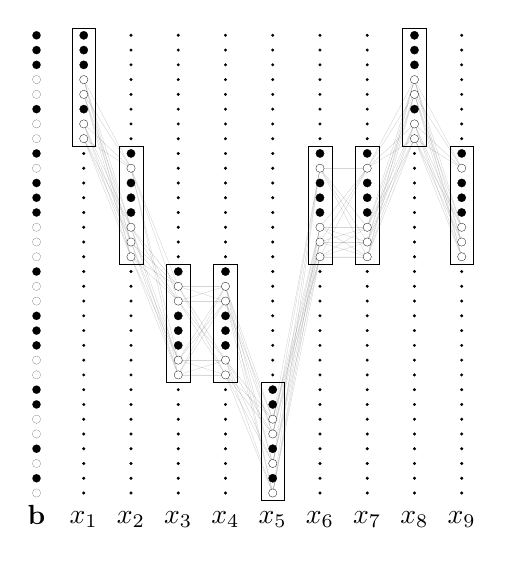
\begin{tikzpicture}%
\path[draw,line width=0.01pt,fill=white,radius=1.5pt] (0.0,0.0) circle;%
\path[draw,line width=0.01pt,fill=black,radius=1.5pt] (0.0,0.1875) circle;%
\path[draw,line width=0.01pt,fill=white,radius=1.5pt] (0.0,0.375) circle;%
\path[draw,line width=0.01pt,fill=black,radius=1.5pt] (0.0,0.5625) circle;%
\path[draw,line width=0.01pt,fill=white,radius=1.5pt] (0.0,0.75) circle;%
\path[draw,line width=0.01pt,fill=white,radius=1.5pt] (0.0,0.9375) circle;%
\path[draw,line width=0.01pt,fill=black,radius=1.5pt] (0.0,1.125) circle;%
\path[draw,line width=0.01pt,fill=black,radius=1.5pt] (0.0,1.3125) circle;%
\path[draw,line width=0.01pt,fill=white,radius=1.5pt] (0.0,1.5) circle;%
\path[draw,line width=0.01pt,fill=white,radius=1.5pt] (0.0,1.6875) circle;%
\path[draw,line width=0.01pt,fill=black,radius=1.5pt] (0.0,1.875) circle;%
\path[draw,line width=0.01pt,fill=black,radius=1.5pt] (0.0,2.0625) circle;%
\path[draw,line width=0.01pt,fill=black,radius=1.5pt] (0.0,2.25) circle;%
\path[draw,line width=0.01pt,fill=white,radius=1.5pt] (0.0,2.4375) circle;%
\path[draw,line width=0.01pt,fill=white,radius=1.5pt] (0.0,2.625) circle;%
\path[draw,line width=0.01pt,fill=black,radius=1.5pt] (0.0,2.8125) circle;%
\path[draw,line width=0.01pt,fill=white,radius=1.5pt] (0.0,3.0) circle;%
\path[draw,line width=0.01pt,fill=white,radius=1.5pt] (0.0,3.1875) circle;%
\path[draw,line width=0.01pt,fill=white,radius=1.5pt] (0.0,3.375) circle;%
\path[draw,line width=0.01pt,fill=black,radius=1.5pt] (0.0,3.5625) circle;%
\path[draw,line width=0.01pt,fill=black,radius=1.5pt] (0.0,3.75) circle;%
\path[draw,line width=0.01pt,fill=black,radius=1.5pt] (0.0,3.9375) circle;%
\path[draw,line width=0.01pt,fill=white,radius=1.5pt] (0.0,4.125) circle;%
\path[draw,line width=0.01pt,fill=black,radius=1.5pt] (0.0,4.3125) circle;%
\path[draw,line width=0.01pt,fill=white,radius=1.5pt] (0.0,4.5) circle;%
\path[draw,line width=0.01pt,fill=white,radius=1.5pt] (0.0,4.6875) circle;%
\path[draw,line width=0.01pt,fill=black,radius=1.5pt] (0.0,4.875) circle;%
\path[draw,line width=0.01pt,fill=white,radius=1.5pt] (0.0,5.0625) circle;%
\path[draw,line width=0.01pt,fill=white,radius=1.5pt] (0.0,5.25) circle;%
\path[draw,line width=0.01pt,fill=black,radius=1.5pt] (0.0,5.4375) circle;%
\path[draw,line width=0.01pt,fill=black,radius=1.5pt] (0.0,5.625) circle;%
\path[draw,line width=0.01pt,fill=black,radius=1.5pt] (0.0,5.8125) circle;%
\path[draw,line width=0.1pt,opacity=0.15,fill=black] (0.6,4.5) -- (1.2,3.0);%
\path[draw,line width=0.1pt,opacity=0.15,fill=black] (0.6,4.5) -- (1.2,3.1875);%
\path[draw,line width=0.1pt,opacity=0.15,fill=black] (0.6,4.5) -- (1.2,3.375);%
\path[draw,line width=0.1pt,opacity=0.15,fill=black] (0.6,4.5) -- (1.2,4.125);%
\path[draw,line width=0.1pt,opacity=0.15,fill=black] (0.6,4.6875) -- (1.2,3.0);%
\path[draw,line width=0.1pt,opacity=0.15,fill=black] (0.6,4.6875) -- (1.2,3.1875);%
\path[draw,line width=0.1pt,opacity=0.15,fill=black] (0.6,4.6875) -- (1.2,3.375);%
\path[draw,line width=0.1pt,opacity=0.15,fill=black] (0.6,4.6875) -- (1.2,4.125);%
\path[draw,line width=0.1pt,opacity=0.15,fill=black] (0.6,5.0625) -- (1.2,3.0);%
\path[draw,line width=0.1pt,opacity=0.15,fill=black] (0.6,5.0625) -- (1.2,3.1875);%
\path[draw,line width=0.1pt,opacity=0.15,fill=black] (0.6,5.0625) -- (1.2,3.375);%
\path[draw,line width=0.1pt,opacity=0.15,fill=black] (0.6,5.0625) -- (1.2,4.125);%
\path[draw,line width=0.1pt,opacity=0.15,fill=black] (0.6,5.25) -- (1.2,3.0);%
\path[draw,line width=0.1pt,opacity=0.15,fill=black] (0.6,5.25) -- (1.2,3.1875);%
\path[draw,line width=0.1pt,opacity=0.15,fill=black] (0.6,5.25) -- (1.2,3.375);%
\path[draw,line width=0.1pt,opacity=0.15,fill=black] (0.6,5.25) -- (1.2,4.125);%
\path[draw,line width=0.1pt,opacity=0.15,fill=black] (1.2,3.0) -- (1.8,1.5);%
\path[draw,line width=0.1pt,opacity=0.15,fill=black] (1.2,3.0) -- (1.8,1.6875);%
\path[draw,line width=0.1pt,opacity=0.15,fill=black] (1.2,3.0) -- (1.8,2.4375);%
\path[draw,line width=0.1pt,opacity=0.15,fill=black] (1.2,3.0) -- (1.8,2.625);%
\path[draw,line width=0.1pt,opacity=0.15,fill=black] (1.2,3.1875) -- (1.8,1.5);%
\path[draw,line width=0.1pt,opacity=0.15,fill=black] (1.2,3.1875) -- (1.8,1.6875);%
\path[draw,line width=0.1pt,opacity=0.15,fill=black] (1.2,3.1875) -- (1.8,2.4375);%
\path[draw,line width=0.1pt,opacity=0.15,fill=black] (1.2,3.1875) -- (1.8,2.625);%
\path[draw,line width=0.1pt,opacity=0.15,fill=black] (1.2,3.375) -- (1.8,1.5);%
\path[draw,line width=0.1pt,opacity=0.15,fill=black] (1.2,3.375) -- (1.8,1.6875);%
\path[draw,line width=0.1pt,opacity=0.15,fill=black] (1.2,3.375) -- (1.8,2.4375);%
\path[draw,line width=0.1pt,opacity=0.15,fill=black] (1.2,3.375) -- (1.8,2.625);%
\path[draw,line width=0.1pt,opacity=0.15,fill=black] (1.2,4.125) -- (1.8,1.5);%
\path[draw,line width=0.1pt,opacity=0.15,fill=black] (1.2,4.125) -- (1.8,1.6875);%
\path[draw,line width=0.1pt,opacity=0.15,fill=black] (1.2,4.125) -- (1.8,2.4375);%
\path[draw,line width=0.1pt,opacity=0.15,fill=black] (1.2,4.125) -- (1.8,2.625);%
\path[draw,line width=0.1pt,opacity=0.15,fill=black] (1.8,1.5) -- (2.4,1.5);%
\path[draw,line width=0.1pt,opacity=0.15,fill=black] (1.8,1.5) -- (2.4,1.6875);%
\path[draw,line width=0.1pt,opacity=0.15,fill=black] (1.8,1.5) -- (2.4,2.4375);%
\path[draw,line width=0.1pt,opacity=0.15,fill=black] (1.8,1.5) -- (2.4,2.625);%
\path[draw,line width=0.1pt,opacity=0.15,fill=black] (1.8,1.6875) -- (2.4,1.5);%
\path[draw,line width=0.1pt,opacity=0.15,fill=black] (1.8,1.6875) -- (2.4,1.6875);%
\path[draw,line width=0.1pt,opacity=0.15,fill=black] (1.8,1.6875) -- (2.4,2.4375);%
\path[draw,line width=0.1pt,opacity=0.15,fill=black] (1.8,1.6875) -- (2.4,2.625);%
\path[draw,line width=0.1pt,opacity=0.15,fill=black] (1.8,2.4375) -- (2.4,1.5);%
\path[draw,line width=0.1pt,opacity=0.15,fill=black] (1.8,2.4375) -- (2.4,1.6875);%
\path[draw,line width=0.1pt,opacity=0.15,fill=black] (1.8,2.4375) -- (2.4,2.4375);%
\path[draw,line width=0.1pt,opacity=0.15,fill=black] (1.8,2.4375) -- (2.4,2.625);%
\path[draw,line width=0.1pt,opacity=0.15,fill=black] (1.8,2.625) -- (2.4,1.5);%
\path[draw,line width=0.1pt,opacity=0.15,fill=black] (1.8,2.625) -- (2.4,1.6875);%
\path[draw,line width=0.1pt,opacity=0.15,fill=black] (1.8,2.625) -- (2.4,2.4375);%
\path[draw,line width=0.1pt,opacity=0.15,fill=black] (1.8,2.625) -- (2.4,2.625);%
\path[draw,line width=0.1pt,opacity=0.15,fill=black] (2.4,1.5) -- (3.0,0.0);%
\path[draw,line width=0.1pt,opacity=0.15,fill=black] (2.4,1.5) -- (3.0,0.375);%
\path[draw,line width=0.1pt,opacity=0.15,fill=black] (2.4,1.5) -- (3.0,0.75);%
\path[draw,line width=0.1pt,opacity=0.15,fill=black] (2.4,1.5) -- (3.0,0.9375);%
\path[draw,line width=0.1pt,opacity=0.15,fill=black] (2.4,1.6875) -- (3.0,0.0);%
\path[draw,line width=0.1pt,opacity=0.15,fill=black] (2.4,1.6875) -- (3.0,0.375);%
\path[draw,line width=0.1pt,opacity=0.15,fill=black] (2.4,1.6875) -- (3.0,0.75);%
\path[draw,line width=0.1pt,opacity=0.15,fill=black] (2.4,1.6875) -- (3.0,0.9375);%
\path[draw,line width=0.1pt,opacity=0.15,fill=black] (2.4,2.4375) -- (3.0,0.0);%
\path[draw,line width=0.1pt,opacity=0.15,fill=black] (2.4,2.4375) -- (3.0,0.375);%
\path[draw,line width=0.1pt,opacity=0.15,fill=black] (2.4,2.4375) -- (3.0,0.75);%
\path[draw,line width=0.1pt,opacity=0.15,fill=black] (2.4,2.4375) -- (3.0,0.9375);%
\path[draw,line width=0.1pt,opacity=0.15,fill=black] (2.4,2.625) -- (3.0,0.0);%
\path[draw,line width=0.1pt,opacity=0.15,fill=black] (2.4,2.625) -- (3.0,0.375);%
\path[draw,line width=0.1pt,opacity=0.15,fill=black] (2.4,2.625) -- (3.0,0.75);%
\path[draw,line width=0.1pt,opacity=0.15,fill=black] (2.4,2.625) -- (3.0,0.9375);%
\path[draw,line width=0.1pt,opacity=0.15,fill=black] (3.0,0.0) -- (3.6,3.0);%
\path[draw,line width=0.1pt,opacity=0.15,fill=black] (3.0,0.0) -- (3.6,3.1875);%
\path[draw,line width=0.1pt,opacity=0.15,fill=black] (3.0,0.0) -- (3.6,3.375);%
\path[draw,line width=0.1pt,opacity=0.15,fill=black] (3.0,0.0) -- (3.6,4.125);%
\path[draw,line width=0.1pt,opacity=0.15,fill=black] (3.0,0.375) -- (3.6,3.0);%
\path[draw,line width=0.1pt,opacity=0.15,fill=black] (3.0,0.375) -- (3.6,3.1875);%
\path[draw,line width=0.1pt,opacity=0.15,fill=black] (3.0,0.375) -- (3.6,3.375);%
\path[draw,line width=0.1pt,opacity=0.15,fill=black] (3.0,0.375) -- (3.6,4.125);%
\path[draw,line width=0.1pt,opacity=0.15,fill=black] (3.0,0.75) -- (3.6,3.0);%
\path[draw,line width=0.1pt,opacity=0.15,fill=black] (3.0,0.75) -- (3.6,3.1875);%
\path[draw,line width=0.1pt,opacity=0.15,fill=black] (3.0,0.75) -- (3.6,3.375);%
\path[draw,line width=0.1pt,opacity=0.15,fill=black] (3.0,0.75) -- (3.6,4.125);%
\path[draw,line width=0.1pt,opacity=0.15,fill=black] (3.0,0.9375) -- (3.6,3.0);%
\path[draw,line width=0.1pt,opacity=0.15,fill=black] (3.0,0.9375) -- (3.6,3.1875);%
\path[draw,line width=0.1pt,opacity=0.15,fill=black] (3.0,0.9375) -- (3.6,3.375);%
\path[draw,line width=0.1pt,opacity=0.15,fill=black] (3.0,0.9375) -- (3.6,4.125);%
\path[draw,line width=0.1pt,opacity=0.15,fill=black] (3.6,3.0) -- (4.2,3.0);%
\path[draw,line width=0.1pt,opacity=0.15,fill=black] (3.6,3.0) -- (4.2,3.1875);%
\path[draw,line width=0.1pt,opacity=0.15,fill=black] (3.6,3.0) -- (4.2,3.375);%
\path[draw,line width=0.1pt,opacity=0.15,fill=black] (3.6,3.0) -- (4.2,4.125);%
\path[draw,line width=0.1pt,opacity=0.15,fill=black] (3.6,3.1875) -- (4.2,3.0);%
\path[draw,line width=0.1pt,opacity=0.15,fill=black] (3.6,3.1875) -- (4.2,3.1875);%
\path[draw,line width=0.1pt,opacity=0.15,fill=black] (3.6,3.1875) -- (4.2,3.375);%
\path[draw,line width=0.1pt,opacity=0.15,fill=black] (3.6,3.1875) -- (4.2,4.125);%
\path[draw,line width=0.1pt,opacity=0.15,fill=black] (3.6,3.375) -- (4.2,3.0);%
\path[draw,line width=0.1pt,opacity=0.15,fill=black] (3.6,3.375) -- (4.2,3.1875);%
\path[draw,line width=0.1pt,opacity=0.15,fill=black] (3.6,3.375) -- (4.2,3.375);%
\path[draw,line width=0.1pt,opacity=0.15,fill=black] (3.6,3.375) -- (4.2,4.125);%
\path[draw,line width=0.1pt,opacity=0.15,fill=black] (3.6,4.125) -- (4.2,3.0);%
\path[draw,line width=0.1pt,opacity=0.15,fill=black] (3.6,4.125) -- (4.2,3.1875);%
\path[draw,line width=0.1pt,opacity=0.15,fill=black] (3.6,4.125) -- (4.2,3.375);%
\path[draw,line width=0.1pt,opacity=0.15,fill=black] (3.6,4.125) -- (4.2,4.125);%
\path[draw,line width=0.1pt,opacity=0.15,fill=black] (4.2,3.0) -- (4.8,4.5);%
\path[draw,line width=0.1pt,opacity=0.15,fill=black] (4.2,3.0) -- (4.8,4.6875);%
\path[draw,line width=0.1pt,opacity=0.15,fill=black] (4.2,3.0) -- (4.8,5.0625);%
\path[draw,line width=0.1pt,opacity=0.15,fill=black] (4.2,3.0) -- (4.8,5.25);%
\path[draw,line width=0.1pt,opacity=0.15,fill=black] (4.2,3.1875) -- (4.8,4.5);%
\path[draw,line width=0.1pt,opacity=0.15,fill=black] (4.2,3.1875) -- (4.8,4.6875);%
\path[draw,line width=0.1pt,opacity=0.15,fill=black] (4.2,3.1875) -- (4.8,5.0625);%
\path[draw,line width=0.1pt,opacity=0.15,fill=black] (4.2,3.1875) -- (4.8,5.25);%
\path[draw,line width=0.1pt,opacity=0.15,fill=black] (4.2,3.375) -- (4.8,4.5);%
\path[draw,line width=0.1pt,opacity=0.15,fill=black] (4.2,3.375) -- (4.8,4.6875);%
\path[draw,line width=0.1pt,opacity=0.15,fill=black] (4.2,3.375) -- (4.8,5.0625);%
\path[draw,line width=0.1pt,opacity=0.15,fill=black] (4.2,3.375) -- (4.8,5.25);%
\path[draw,line width=0.1pt,opacity=0.15,fill=black] (4.2,4.125) -- (4.8,4.5);%
\path[draw,line width=0.1pt,opacity=0.15,fill=black] (4.2,4.125) -- (4.8,4.6875);%
\path[draw,line width=0.1pt,opacity=0.15,fill=black] (4.2,4.125) -- (4.8,5.0625);%
\path[draw,line width=0.1pt,opacity=0.15,fill=black] (4.2,4.125) -- (4.8,5.25);%
\path[draw,line width=0.1pt,opacity=0.15,fill=black] (4.8,4.5) -- (5.4,3.0);%
\path[draw,line width=0.1pt,opacity=0.15,fill=black] (4.8,4.5) -- (5.4,3.1875);%
\path[draw,line width=0.1pt,opacity=0.15,fill=black] (4.8,4.5) -- (5.4,3.375);%
\path[draw,line width=0.1pt,opacity=0.15,fill=black] (4.8,4.5) -- (5.4,4.125);%
\path[draw,line width=0.1pt,opacity=0.15,fill=black] (4.8,4.6875) -- (5.4,3.0);%
\path[draw,line width=0.1pt,opacity=0.15,fill=black] (4.8,4.6875) -- (5.4,3.1875);%
\path[draw,line width=0.1pt,opacity=0.15,fill=black] (4.8,4.6875) -- (5.4,3.375);%
\path[draw,line width=0.1pt,opacity=0.15,fill=black] (4.8,4.6875) -- (5.4,4.125);%
\path[draw,line width=0.1pt,opacity=0.15,fill=black] (4.8,5.0625) -- (5.4,3.0);%
\path[draw,line width=0.1pt,opacity=0.15,fill=black] (4.8,5.0625) -- (5.4,3.1875);%
\path[draw,line width=0.1pt,opacity=0.15,fill=black] (4.8,5.0625) -- (5.4,3.375);%
\path[draw,line width=0.1pt,opacity=0.15,fill=black] (4.8,5.0625) -- (5.4,4.125);%
\path[draw,line width=0.1pt,opacity=0.15,fill=black] (4.8,5.25) -- (5.4,3.0);%
\path[draw,line width=0.1pt,opacity=0.15,fill=black] (4.8,5.25) -- (5.4,3.1875);%
\path[draw,line width=0.1pt,opacity=0.15,fill=black] (4.8,5.25) -- (5.4,3.375);%
\path[draw,line width=0.1pt,opacity=0.15,fill=black] (4.8,5.25) -- (5.4,4.125);%
\path[draw,line width=0.2pt] (0.45,4.40625) rectangle (0.75,5.90625);%
\path[draw,line width=0.2pt] (1.05,2.90625) rectangle (1.35,4.40625);%
\path[draw,line width=0.2pt] (1.65,1.40625) rectangle (1.95,2.90625);%
\path[draw,line width=0.2pt] (2.25,1.40625) rectangle (2.55,2.90625);%
\path[draw,line width=0.2pt] (2.85,-0.09375) rectangle (3.15,1.40625);%
\path[draw,line width=0.2pt] (3.45,2.90625) rectangle (3.75,4.40625);%
\path[draw,line width=0.2pt] (4.05,2.90625) rectangle (4.35,4.40625);%
\path[draw,line width=0.2pt] (4.65,4.40625) rectangle (4.95,5.90625);%
\path[draw,line width=0.2pt] (5.25,2.90625) rectangle (5.55,4.40625);%
\node[inner sep=0] (b) at (0.0,-0.28125) {$\mathbf{b}$};%
\node (x1) at (0.6,-0.3375) {$x_1$};%
\node (x2) at (1.2,-0.3375) {$x_2$};%
\node (x3) at (1.8,-0.3375) {$x_3$};%
\node (x4) at (2.4,-0.3375) {$x_4$};%
\node (x5) at (3.0,-0.3375) {$x_5$};%
\node (x6) at (3.6,-0.3375) {$x_6$};%
\node (x7) at (4.2,-0.3375) {$x_7$};%
\node (x8) at (4.8,-0.3375) {$x_8$};%
\node (x9) at (5.4,-0.3375) {$x_9$};%
\path[draw,line width=0.1pt,fill=black,radius=0.5pt] (0.6,0.0) circle;%
\path[draw,line width=0.1pt,fill=black,radius=0.5pt] (0.6,0.1875) circle;%
\path[draw,line width=0.1pt,fill=black,radius=0.5pt] (0.6,0.375) circle;%
\path[draw,line width=0.1pt,fill=black,radius=0.5pt] (0.6,0.5625) circle;%
\path[draw,line width=0.1pt,fill=black,radius=0.5pt] (0.6,0.75) circle;%
\path[draw,line width=0.1pt,fill=black,radius=0.5pt] (0.6,0.9375) circle;%
\path[draw,line width=0.1pt,fill=black,radius=0.5pt] (0.6,1.125) circle;%
\path[draw,line width=0.1pt,fill=black,radius=0.5pt] (0.6,1.3125) circle;%
\path[draw,line width=0.1pt,fill=black,radius=0.5pt] (0.6,1.5) circle;%
\path[draw,line width=0.1pt,fill=black,radius=0.5pt] (0.6,1.6875) circle;%
\path[draw,line width=0.1pt,fill=black,radius=0.5pt] (0.6,1.875) circle;%
\path[draw,line width=0.1pt,fill=black,radius=0.5pt] (0.6,2.0625) circle;%
\path[draw,line width=0.1pt,fill=black,radius=0.5pt] (0.6,2.25) circle;%
\path[draw,line width=0.1pt,fill=black,radius=0.5pt] (0.6,2.4375) circle;%
\path[draw,line width=0.1pt,fill=black,radius=0.5pt] (0.6,2.625) circle;%
\path[draw,line width=0.1pt,fill=black,radius=0.5pt] (0.6,2.8125) circle;%
\path[draw,line width=0.1pt,fill=black,radius=0.5pt] (0.6,3.0) circle;%
\path[draw,line width=0.1pt,fill=black,radius=0.5pt] (0.6,3.1875) circle;%
\path[draw,line width=0.1pt,fill=black,radius=0.5pt] (0.6,3.375) circle;%
\path[draw,line width=0.1pt,fill=black,radius=0.5pt] (0.6,3.5625) circle;%
\path[draw,line width=0.1pt,fill=black,radius=0.5pt] (0.6,3.75) circle;%
\path[draw,line width=0.1pt,fill=black,radius=0.5pt] (0.6,3.9375) circle;%
\path[draw,line width=0.1pt,fill=black,radius=0.5pt] (0.6,4.125) circle;%
\path[draw,line width=0.1pt,fill=black,radius=0.5pt] (0.6,4.3125) circle;%
\path[draw,line width=0.1pt,fill=white,radius=1.5pt] (0.6,4.5) circle;%
\path[draw,line width=0.1pt,fill=white,radius=1.5pt] (0.6,4.6875) circle;%
\path[draw,line width=0.1pt,fill=black,radius=1.5pt] (0.6,4.875) circle;%
\path[draw,line width=0.1pt,fill=white,radius=1.5pt] (0.6,5.0625) circle;%
\path[draw,line width=0.1pt,fill=white,radius=1.5pt] (0.6,5.25) circle;%
\path[draw,line width=0.1pt,fill=black,radius=1.5pt] (0.6,5.4375) circle;%
\path[draw,line width=0.1pt,fill=black,radius=1.5pt] (0.6,5.625) circle;%
\path[draw,line width=0.1pt,fill=black,radius=1.5pt] (0.6,5.8125) circle;%
\path[draw,line width=0.1pt,fill=black,radius=0.5pt] (1.2,0.0) circle;%
\path[draw,line width=0.1pt,fill=black,radius=0.5pt] (1.2,0.1875) circle;%
\path[draw,line width=0.1pt,fill=black,radius=0.5pt] (1.2,0.375) circle;%
\path[draw,line width=0.1pt,fill=black,radius=0.5pt] (1.2,0.5625) circle;%
\path[draw,line width=0.1pt,fill=black,radius=0.5pt] (1.2,0.75) circle;%
\path[draw,line width=0.1pt,fill=black,radius=0.5pt] (1.2,0.9375) circle;%
\path[draw,line width=0.1pt,fill=black,radius=0.5pt] (1.2,1.125) circle;%
\path[draw,line width=0.1pt,fill=black,radius=0.5pt] (1.2,1.3125) circle;%
\path[draw,line width=0.1pt,fill=black,radius=0.5pt] (1.2,1.5) circle;%
\path[draw,line width=0.1pt,fill=black,radius=0.5pt] (1.2,1.6875) circle;%
\path[draw,line width=0.1pt,fill=black,radius=0.5pt] (1.2,1.875) circle;%
\path[draw,line width=0.1pt,fill=black,radius=0.5pt] (1.2,2.0625) circle;%
\path[draw,line width=0.1pt,fill=black,radius=0.5pt] (1.2,2.25) circle;%
\path[draw,line width=0.1pt,fill=black,radius=0.5pt] (1.2,2.4375) circle;%
\path[draw,line width=0.1pt,fill=black,radius=0.5pt] (1.2,2.625) circle;%
\path[draw,line width=0.1pt,fill=black,radius=0.5pt] (1.2,2.8125) circle;%
\path[draw,line width=0.1pt,fill=white,radius=1.5pt] (1.2,3.0) circle;%
\path[draw,line width=0.1pt,fill=white,radius=1.5pt] (1.2,3.1875) circle;%
\path[draw,line width=0.1pt,fill=white,radius=1.5pt] (1.2,3.375) circle;%
\path[draw,line width=0.1pt,fill=black,radius=1.5pt] (1.2,3.5625) circle;%
\path[draw,line width=0.1pt,fill=black,radius=1.5pt] (1.2,3.75) circle;%
\path[draw,line width=0.1pt,fill=black,radius=1.5pt] (1.2,3.9375) circle;%
\path[draw,line width=0.1pt,fill=white,radius=1.5pt] (1.2,4.125) circle;%
\path[draw,line width=0.1pt,fill=black,radius=1.5pt] (1.2,4.3125) circle;%
\path[draw,line width=0.1pt,fill=black,radius=0.5pt] (1.2,4.5) circle;%
\path[draw,line width=0.1pt,fill=black,radius=0.5pt] (1.2,4.6875) circle;%
\path[draw,line width=0.1pt,fill=black,radius=0.5pt] (1.2,4.875) circle;%
\path[draw,line width=0.1pt,fill=black,radius=0.5pt] (1.2,5.0625) circle;%
\path[draw,line width=0.1pt,fill=black,radius=0.5pt] (1.2,5.25) circle;%
\path[draw,line width=0.1pt,fill=black,radius=0.5pt] (1.2,5.4375) circle;%
\path[draw,line width=0.1pt,fill=black,radius=0.5pt] (1.2,5.625) circle;%
\path[draw,line width=0.1pt,fill=black,radius=0.5pt] (1.2,5.8125) circle;%
\path[draw,line width=0.1pt,fill=black,radius=0.5pt] (1.8,0.0) circle;%
\path[draw,line width=0.1pt,fill=black,radius=0.5pt] (1.8,0.1875) circle;%
\path[draw,line width=0.1pt,fill=black,radius=0.5pt] (1.8,0.375) circle;%
\path[draw,line width=0.1pt,fill=black,radius=0.5pt] (1.8,0.5625) circle;%
\path[draw,line width=0.1pt,fill=black,radius=0.5pt] (1.8,0.75) circle;%
\path[draw,line width=0.1pt,fill=black,radius=0.5pt] (1.8,0.9375) circle;%
\path[draw,line width=0.1pt,fill=black,radius=0.5pt] (1.8,1.125) circle;%
\path[draw,line width=0.1pt,fill=black,radius=0.5pt] (1.8,1.3125) circle;%
\path[draw,line width=0.1pt,fill=white,radius=1.5pt] (1.8,1.5) circle;%
\path[draw,line width=0.1pt,fill=white,radius=1.5pt] (1.8,1.6875) circle;%
\path[draw,line width=0.1pt,fill=black,radius=1.5pt] (1.8,1.875) circle;%
\path[draw,line width=0.1pt,fill=black,radius=1.5pt] (1.8,2.0625) circle;%
\path[draw,line width=0.1pt,fill=black,radius=1.5pt] (1.8,2.25) circle;%
\path[draw,line width=0.1pt,fill=white,radius=1.5pt] (1.8,2.4375) circle;%
\path[draw,line width=0.1pt,fill=white,radius=1.5pt] (1.8,2.625) circle;%
\path[draw,line width=0.1pt,fill=black,radius=1.5pt] (1.8,2.8125) circle;%
\path[draw,line width=0.1pt,fill=black,radius=0.5pt] (1.8,3.0) circle;%
\path[draw,line width=0.1pt,fill=black,radius=0.5pt] (1.8,3.1875) circle;%
\path[draw,line width=0.1pt,fill=black,radius=0.5pt] (1.8,3.375) circle;%
\path[draw,line width=0.1pt,fill=black,radius=0.5pt] (1.8,3.5625) circle;%
\path[draw,line width=0.1pt,fill=black,radius=0.5pt] (1.8,3.75) circle;%
\path[draw,line width=0.1pt,fill=black,radius=0.5pt] (1.8,3.9375) circle;%
\path[draw,line width=0.1pt,fill=black,radius=0.5pt] (1.8,4.125) circle;%
\path[draw,line width=0.1pt,fill=black,radius=0.5pt] (1.8,4.3125) circle;%
\path[draw,line width=0.1pt,fill=black,radius=0.5pt] (1.8,4.5) circle;%
\path[draw,line width=0.1pt,fill=black,radius=0.5pt] (1.8,4.6875) circle;%
\path[draw,line width=0.1pt,fill=black,radius=0.5pt] (1.8,4.875) circle;%
\path[draw,line width=0.1pt,fill=black,radius=0.5pt] (1.8,5.0625) circle;%
\path[draw,line width=0.1pt,fill=black,radius=0.5pt] (1.8,5.25) circle;%
\path[draw,line width=0.1pt,fill=black,radius=0.5pt] (1.8,5.4375) circle;%
\path[draw,line width=0.1pt,fill=black,radius=0.5pt] (1.8,5.625) circle;%
\path[draw,line width=0.1pt,fill=black,radius=0.5pt] (1.8,5.8125) circle;%
\path[draw,line width=0.1pt,fill=black,radius=0.5pt] (2.4,0.0) circle;%
\path[draw,line width=0.1pt,fill=black,radius=0.5pt] (2.4,0.1875) circle;%
\path[draw,line width=0.1pt,fill=black,radius=0.5pt] (2.4,0.375) circle;%
\path[draw,line width=0.1pt,fill=black,radius=0.5pt] (2.4,0.5625) circle;%
\path[draw,line width=0.1pt,fill=black,radius=0.5pt] (2.4,0.75) circle;%
\path[draw,line width=0.1pt,fill=black,radius=0.5pt] (2.4,0.9375) circle;%
\path[draw,line width=0.1pt,fill=black,radius=0.5pt] (2.4,1.125) circle;%
\path[draw,line width=0.1pt,fill=black,radius=0.5pt] (2.4,1.3125) circle;%
\path[draw,line width=0.1pt,fill=white,radius=1.5pt] (2.4,1.5) circle;%
\path[draw,line width=0.1pt,fill=white,radius=1.5pt] (2.4,1.6875) circle;%
\path[draw,line width=0.1pt,fill=black,radius=1.5pt] (2.4,1.875) circle;%
\path[draw,line width=0.1pt,fill=black,radius=1.5pt] (2.4,2.0625) circle;%
\path[draw,line width=0.1pt,fill=black,radius=1.5pt] (2.4,2.25) circle;%
\path[draw,line width=0.1pt,fill=white,radius=1.5pt] (2.4,2.4375) circle;%
\path[draw,line width=0.1pt,fill=white,radius=1.5pt] (2.4,2.625) circle;%
\path[draw,line width=0.1pt,fill=black,radius=1.5pt] (2.4,2.8125) circle;%
\path[draw,line width=0.1pt,fill=black,radius=0.5pt] (2.4,3.0) circle;%
\path[draw,line width=0.1pt,fill=black,radius=0.5pt] (2.4,3.1875) circle;%
\path[draw,line width=0.1pt,fill=black,radius=0.5pt] (2.4,3.375) circle;%
\path[draw,line width=0.1pt,fill=black,radius=0.5pt] (2.4,3.5625) circle;%
\path[draw,line width=0.1pt,fill=black,radius=0.5pt] (2.4,3.75) circle;%
\path[draw,line width=0.1pt,fill=black,radius=0.5pt] (2.4,3.9375) circle;%
\path[draw,line width=0.1pt,fill=black,radius=0.5pt] (2.4,4.125) circle;%
\path[draw,line width=0.1pt,fill=black,radius=0.5pt] (2.4,4.3125) circle;%
\path[draw,line width=0.1pt,fill=black,radius=0.5pt] (2.4,4.5) circle;%
\path[draw,line width=0.1pt,fill=black,radius=0.5pt] (2.4,4.6875) circle;%
\path[draw,line width=0.1pt,fill=black,radius=0.5pt] (2.4,4.875) circle;%
\path[draw,line width=0.1pt,fill=black,radius=0.5pt] (2.4,5.0625) circle;%
\path[draw,line width=0.1pt,fill=black,radius=0.5pt] (2.4,5.25) circle;%
\path[draw,line width=0.1pt,fill=black,radius=0.5pt] (2.4,5.4375) circle;%
\path[draw,line width=0.1pt,fill=black,radius=0.5pt] (2.4,5.625) circle;%
\path[draw,line width=0.1pt,fill=black,radius=0.5pt] (2.4,5.8125) circle;%
\path[draw,line width=0.1pt,fill=white,radius=1.5pt] (3.0,0.0) circle;%
\path[draw,line width=0.1pt,fill=black,radius=1.5pt] (3.0,0.1875) circle;%
\path[draw,line width=0.1pt,fill=white,radius=1.5pt] (3.0,0.375) circle;%
\path[draw,line width=0.1pt,fill=black,radius=1.5pt] (3.0,0.5625) circle;%
\path[draw,line width=0.1pt,fill=white,radius=1.5pt] (3.0,0.75) circle;%
\path[draw,line width=0.1pt,fill=white,radius=1.5pt] (3.0,0.9375) circle;%
\path[draw,line width=0.1pt,fill=black,radius=1.5pt] (3.0,1.125) circle;%
\path[draw,line width=0.1pt,fill=black,radius=1.5pt] (3.0,1.3125) circle;%
\path[draw,line width=0.1pt,fill=black,radius=0.5pt] (3.0,1.5) circle;%
\path[draw,line width=0.1pt,fill=black,radius=0.5pt] (3.0,1.6875) circle;%
\path[draw,line width=0.1pt,fill=black,radius=0.5pt] (3.0,1.875) circle;%
\path[draw,line width=0.1pt,fill=black,radius=0.5pt] (3.0,2.0625) circle;%
\path[draw,line width=0.1pt,fill=black,radius=0.5pt] (3.0,2.25) circle;%
\path[draw,line width=0.1pt,fill=black,radius=0.5pt] (3.0,2.4375) circle;%
\path[draw,line width=0.1pt,fill=black,radius=0.5pt] (3.0,2.625) circle;%
\path[draw,line width=0.1pt,fill=black,radius=0.5pt] (3.0,2.8125) circle;%
\path[draw,line width=0.1pt,fill=black,radius=0.5pt] (3.0,3.0) circle;%
\path[draw,line width=0.1pt,fill=black,radius=0.5pt] (3.0,3.1875) circle;%
\path[draw,line width=0.1pt,fill=black,radius=0.5pt] (3.0,3.375) circle;%
\path[draw,line width=0.1pt,fill=black,radius=0.5pt] (3.0,3.5625) circle;%
\path[draw,line width=0.1pt,fill=black,radius=0.5pt] (3.0,3.75) circle;%
\path[draw,line width=0.1pt,fill=black,radius=0.5pt] (3.0,3.9375) circle;%
\path[draw,line width=0.1pt,fill=black,radius=0.5pt] (3.0,4.125) circle;%
\path[draw,line width=0.1pt,fill=black,radius=0.5pt] (3.0,4.3125) circle;%
\path[draw,line width=0.1pt,fill=black,radius=0.5pt] (3.0,4.5) circle;%
\path[draw,line width=0.1pt,fill=black,radius=0.5pt] (3.0,4.6875) circle;%
\path[draw,line width=0.1pt,fill=black,radius=0.5pt] (3.0,4.875) circle;%
\path[draw,line width=0.1pt,fill=black,radius=0.5pt] (3.0,5.0625) circle;%
\path[draw,line width=0.1pt,fill=black,radius=0.5pt] (3.0,5.25) circle;%
\path[draw,line width=0.1pt,fill=black,radius=0.5pt] (3.0,5.4375) circle;%
\path[draw,line width=0.1pt,fill=black,radius=0.5pt] (3.0,5.625) circle;%
\path[draw,line width=0.1pt,fill=black,radius=0.5pt] (3.0,5.8125) circle;%
\path[draw,line width=0.1pt,fill=black,radius=0.5pt] (3.6,0.0) circle;%
\path[draw,line width=0.1pt,fill=black,radius=0.5pt] (3.6,0.1875) circle;%
\path[draw,line width=0.1pt,fill=black,radius=0.5pt] (3.6,0.375) circle;%
\path[draw,line width=0.1pt,fill=black,radius=0.5pt] (3.6,0.5625) circle;%
\path[draw,line width=0.1pt,fill=black,radius=0.5pt] (3.6,0.75) circle;%
\path[draw,line width=0.1pt,fill=black,radius=0.5pt] (3.6,0.9375) circle;%
\path[draw,line width=0.1pt,fill=black,radius=0.5pt] (3.6,1.125) circle;%
\path[draw,line width=0.1pt,fill=black,radius=0.5pt] (3.6,1.3125) circle;%
\path[draw,line width=0.1pt,fill=black,radius=0.5pt] (3.6,1.5) circle;%
\path[draw,line width=0.1pt,fill=black,radius=0.5pt] (3.6,1.6875) circle;%
\path[draw,line width=0.1pt,fill=black,radius=0.5pt] (3.6,1.875) circle;%
\path[draw,line width=0.1pt,fill=black,radius=0.5pt] (3.6,2.0625) circle;%
\path[draw,line width=0.1pt,fill=black,radius=0.5pt] (3.6,2.25) circle;%
\path[draw,line width=0.1pt,fill=black,radius=0.5pt] (3.6,2.4375) circle;%
\path[draw,line width=0.1pt,fill=black,radius=0.5pt] (3.6,2.625) circle;%
\path[draw,line width=0.1pt,fill=black,radius=0.5pt] (3.6,2.8125) circle;%
\path[draw,line width=0.1pt,fill=white,radius=1.5pt] (3.6,3.0) circle;%
\path[draw,line width=0.1pt,fill=white,radius=1.5pt] (3.6,3.1875) circle;%
\path[draw,line width=0.1pt,fill=white,radius=1.5pt] (3.6,3.375) circle;%
\path[draw,line width=0.1pt,fill=black,radius=1.5pt] (3.6,3.5625) circle;%
\path[draw,line width=0.1pt,fill=black,radius=1.5pt] (3.6,3.75) circle;%
\path[draw,line width=0.1pt,fill=black,radius=1.5pt] (3.6,3.9375) circle;%
\path[draw,line width=0.1pt,fill=white,radius=1.5pt] (3.6,4.125) circle;%
\path[draw,line width=0.1pt,fill=black,radius=1.5pt] (3.6,4.3125) circle;%
\path[draw,line width=0.1pt,fill=black,radius=0.5pt] (3.6,4.5) circle;%
\path[draw,line width=0.1pt,fill=black,radius=0.5pt] (3.6,4.6875) circle;%
\path[draw,line width=0.1pt,fill=black,radius=0.5pt] (3.6,4.875) circle;%
\path[draw,line width=0.1pt,fill=black,radius=0.5pt] (3.6,5.0625) circle;%
\path[draw,line width=0.1pt,fill=black,radius=0.5pt] (3.6,5.25) circle;%
\path[draw,line width=0.1pt,fill=black,radius=0.5pt] (3.6,5.4375) circle;%
\path[draw,line width=0.1pt,fill=black,radius=0.5pt] (3.6,5.625) circle;%
\path[draw,line width=0.1pt,fill=black,radius=0.5pt] (3.6,5.8125) circle;%
\path[draw,line width=0.1pt,fill=black,radius=0.5pt] (4.2,0.0) circle;%
\path[draw,line width=0.1pt,fill=black,radius=0.5pt] (4.2,0.1875) circle;%
\path[draw,line width=0.1pt,fill=black,radius=0.5pt] (4.2,0.375) circle;%
\path[draw,line width=0.1pt,fill=black,radius=0.5pt] (4.2,0.5625) circle;%
\path[draw,line width=0.1pt,fill=black,radius=0.5pt] (4.2,0.75) circle;%
\path[draw,line width=0.1pt,fill=black,radius=0.5pt] (4.2,0.9375) circle;%
\path[draw,line width=0.1pt,fill=black,radius=0.5pt] (4.2,1.125) circle;%
\path[draw,line width=0.1pt,fill=black,radius=0.5pt] (4.2,1.3125) circle;%
\path[draw,line width=0.1pt,fill=black,radius=0.5pt] (4.2,1.5) circle;%
\path[draw,line width=0.1pt,fill=black,radius=0.5pt] (4.2,1.6875) circle;%
\path[draw,line width=0.1pt,fill=black,radius=0.5pt] (4.2,1.875) circle;%
\path[draw,line width=0.1pt,fill=black,radius=0.5pt] (4.2,2.0625) circle;%
\path[draw,line width=0.1pt,fill=black,radius=0.5pt] (4.2,2.25) circle;%
\path[draw,line width=0.1pt,fill=black,radius=0.5pt] (4.2,2.4375) circle;%
\path[draw,line width=0.1pt,fill=black,radius=0.5pt] (4.2,2.625) circle;%
\path[draw,line width=0.1pt,fill=black,radius=0.5pt] (4.2,2.8125) circle;%
\path[draw,line width=0.1pt,fill=white,radius=1.5pt] (4.2,3.0) circle;%
\path[draw,line width=0.1pt,fill=white,radius=1.5pt] (4.2,3.1875) circle;%
\path[draw,line width=0.1pt,fill=white,radius=1.5pt] (4.2,3.375) circle;%
\path[draw,line width=0.1pt,fill=black,radius=1.5pt] (4.2,3.5625) circle;%
\path[draw,line width=0.1pt,fill=black,radius=1.5pt] (4.2,3.75) circle;%
\path[draw,line width=0.1pt,fill=black,radius=1.5pt] (4.2,3.9375) circle;%
\path[draw,line width=0.1pt,fill=white,radius=1.5pt] (4.2,4.125) circle;%
\path[draw,line width=0.1pt,fill=black,radius=1.5pt] (4.2,4.3125) circle;%
\path[draw,line width=0.1pt,fill=black,radius=0.5pt] (4.2,4.5) circle;%
\path[draw,line width=0.1pt,fill=black,radius=0.5pt] (4.2,4.6875) circle;%
\path[draw,line width=0.1pt,fill=black,radius=0.5pt] (4.2,4.875) circle;%
\path[draw,line width=0.1pt,fill=black,radius=0.5pt] (4.2,5.0625) circle;%
\path[draw,line width=0.1pt,fill=black,radius=0.5pt] (4.2,5.25) circle;%
\path[draw,line width=0.1pt,fill=black,radius=0.5pt] (4.2,5.4375) circle;%
\path[draw,line width=0.1pt,fill=black,radius=0.5pt] (4.2,5.625) circle;%
\path[draw,line width=0.1pt,fill=black,radius=0.5pt] (4.2,5.8125) circle;%
\path[draw,line width=0.1pt,fill=black,radius=0.5pt] (4.8,0.0) circle;%
\path[draw,line width=0.1pt,fill=black,radius=0.5pt] (4.8,0.1875) circle;%
\path[draw,line width=0.1pt,fill=black,radius=0.5pt] (4.8,0.375) circle;%
\path[draw,line width=0.1pt,fill=black,radius=0.5pt] (4.8,0.5625) circle;%
\path[draw,line width=0.1pt,fill=black,radius=0.5pt] (4.8,0.75) circle;%
\path[draw,line width=0.1pt,fill=black,radius=0.5pt] (4.8,0.9375) circle;%
\path[draw,line width=0.1pt,fill=black,radius=0.5pt] (4.8,1.125) circle;%
\path[draw,line width=0.1pt,fill=black,radius=0.5pt] (4.8,1.3125) circle;%
\path[draw,line width=0.1pt,fill=black,radius=0.5pt] (4.8,1.5) circle;%
\path[draw,line width=0.1pt,fill=black,radius=0.5pt] (4.8,1.6875) circle;%
\path[draw,line width=0.1pt,fill=black,radius=0.5pt] (4.8,1.875) circle;%
\path[draw,line width=0.1pt,fill=black,radius=0.5pt] (4.8,2.0625) circle;%
\path[draw,line width=0.1pt,fill=black,radius=0.5pt] (4.8,2.25) circle;%
\path[draw,line width=0.1pt,fill=black,radius=0.5pt] (4.8,2.4375) circle;%
\path[draw,line width=0.1pt,fill=black,radius=0.5pt] (4.8,2.625) circle;%
\path[draw,line width=0.1pt,fill=black,radius=0.5pt] (4.8,2.8125) circle;%
\path[draw,line width=0.1pt,fill=black,radius=0.5pt] (4.8,3.0) circle;%
\path[draw,line width=0.1pt,fill=black,radius=0.5pt] (4.8,3.1875) circle;%
\path[draw,line width=0.1pt,fill=black,radius=0.5pt] (4.8,3.375) circle;%
\path[draw,line width=0.1pt,fill=black,radius=0.5pt] (4.8,3.5625) circle;%
\path[draw,line width=0.1pt,fill=black,radius=0.5pt] (4.8,3.75) circle;%
\path[draw,line width=0.1pt,fill=black,radius=0.5pt] (4.8,3.9375) circle;%
\path[draw,line width=0.1pt,fill=black,radius=0.5pt] (4.8,4.125) circle;%
\path[draw,line width=0.1pt,fill=black,radius=0.5pt] (4.8,4.3125) circle;%
\path[draw,line width=0.1pt,fill=white,radius=1.5pt] (4.8,4.5) circle;%
\path[draw,line width=0.1pt,fill=white,radius=1.5pt] (4.8,4.6875) circle;%
\path[draw,line width=0.1pt,fill=black,radius=1.5pt] (4.8,4.875) circle;%
\path[draw,line width=0.1pt,fill=white,radius=1.5pt] (4.8,5.0625) circle;%
\path[draw,line width=0.1pt,fill=white,radius=1.5pt] (4.8,5.25) circle;%
\path[draw,line width=0.1pt,fill=black,radius=1.5pt] (4.8,5.4375) circle;%
\path[draw,line width=0.1pt,fill=black,radius=1.5pt] (4.8,5.625) circle;%
\path[draw,line width=0.1pt,fill=black,radius=1.5pt] (4.8,5.8125) circle;%
\path[draw,line width=0.1pt,fill=black,radius=0.5pt] (5.4,0.0) circle;%
\path[draw,line width=0.1pt,fill=black,radius=0.5pt] (5.4,0.1875) circle;%
\path[draw,line width=0.1pt,fill=black,radius=0.5pt] (5.4,0.375) circle;%
\path[draw,line width=0.1pt,fill=black,radius=0.5pt] (5.4,0.5625) circle;%
\path[draw,line width=0.1pt,fill=black,radius=0.5pt] (5.4,0.75) circle;%
\path[draw,line width=0.1pt,fill=black,radius=0.5pt] (5.4,0.9375) circle;%
\path[draw,line width=0.1pt,fill=black,radius=0.5pt] (5.4,1.125) circle;%
\path[draw,line width=0.1pt,fill=black,radius=0.5pt] (5.4,1.3125) circle;%
\path[draw,line width=0.1pt,fill=black,radius=0.5pt] (5.4,1.5) circle;%
\path[draw,line width=0.1pt,fill=black,radius=0.5pt] (5.4,1.6875) circle;%
\path[draw,line width=0.1pt,fill=black,radius=0.5pt] (5.4,1.875) circle;%
\path[draw,line width=0.1pt,fill=black,radius=0.5pt] (5.4,2.0625) circle;%
\path[draw,line width=0.1pt,fill=black,radius=0.5pt] (5.4,2.25) circle;%
\path[draw,line width=0.1pt,fill=black,radius=0.5pt] (5.4,2.4375) circle;%
\path[draw,line width=0.1pt,fill=black,radius=0.5pt] (5.4,2.625) circle;%
\path[draw,line width=0.1pt,fill=black,radius=0.5pt] (5.4,2.8125) circle;%
\path[draw,line width=0.1pt,fill=white,radius=1.5pt] (5.4,3.0) circle;%
\path[draw,line width=0.1pt,fill=white,radius=1.5pt] (5.4,3.1875) circle;%
\path[draw,line width=0.1pt,fill=white,radius=1.5pt] (5.4,3.375) circle;%
\path[draw,line width=0.1pt,fill=black,radius=1.5pt] (5.4,3.5625) circle;%
\path[draw,line width=0.1pt,fill=black,radius=1.5pt] (5.4,3.75) circle;%
\path[draw,line width=0.1pt,fill=black,radius=1.5pt] (5.4,3.9375) circle;%
\path[draw,line width=0.1pt,fill=white,radius=1.5pt] (5.4,4.125) circle;%
\path[draw,line width=0.1pt,fill=black,radius=1.5pt] (5.4,4.3125) circle;%
\path[draw,line width=0.1pt,fill=black,radius=0.5pt] (5.4,4.5) circle;%
\path[draw,line width=0.1pt,fill=black,radius=0.5pt] (5.4,4.6875) circle;%
\path[draw,line width=0.1pt,fill=black,radius=0.5pt] (5.4,4.875) circle;%
\path[draw,line width=0.1pt,fill=black,radius=0.5pt] (5.4,5.0625) circle;%
\path[draw,line width=0.1pt,fill=black,radius=0.5pt] (5.4,5.25) circle;%
\path[draw,line width=0.1pt,fill=black,radius=0.5pt] (5.4,5.4375) circle;%
\path[draw,line width=0.1pt,fill=black,radius=0.5pt] (5.4,5.625) circle;%
\path[draw,line width=0.1pt,fill=black,radius=0.5pt] (5.4,5.8125) circle;%
\end{tikzpicture}%

\end{center}
\caption{
\label{fig:trellis}
A depiction of the trellis for marginal inference
after applying emission sparsity constraints and the state dropout method.
The leftmost column depicts the state dropout mask $\mathbf{b}$,
which is used to prevent states from being considered during inference.
For every token $x_t$, the only incoming edges with nonzero mass are those
whose source was not dropped out, i.e. $b_{z_t} = 1$,
and is within the previous partition, i.e. $z_{t-1}\in\mcC_{x_{t-1}}$.
}
\end{figure}

\subsection{Dropout as State Reduction}
Although a neural parameterization has empirically been shown to find good optima,
it requires that the distributional parameters be recomputed every time the
model parameters are updated.
This entails running a neural network $O(|\mcZ| + |\mcX|)$ times 
at every iteration of gradient descent.

We introduce a variant of dropout called state dropout that lessens
the computational burden of the neural parameterization at training time
while also encouraging full use of the state space and 
reducing the complexity of marginalization.

State dropout prevents a state $z$ from being considered during training.
This can be implemented by adding another constraint to the emission matrix.
Recall distributional parameters of the emission matrix
$\phi \in \mathbb{R}^{|\mcX|\times|\mcZ|}$
and the emission sparsity constraints which associate each token $x$
with a set of states $\mcC_x$.
State dropout samples a mask over states $\mathbf{b} \in \set{0,1}^{|\mcZ|}$.
Given the mask and the emission constraints
defined in the previous section,
we have the following emission distribution:
\begin{equation}
\label{eqn:state_dropout}
p(x \mid z) \propto b_{z}1(z \in \mcC_x)e^{\phi_{xz}}
\end{equation}
Performing marginal inference with state dropout requires $O(Tn^2)$ computation,
where $n$ is the number of nonzero elements of $\mathbf{b}_\mcC, \forall \mcC$.
Additionally, we do not need to compute the parameters of the
transition and emission distributions that have been dropped. 
This reduces the cost of computing $\phi$ and $\psi$ from
$O(|\mcZ|^2+|\mcZ||\mcX|)$ to $n^2 + n|\mcX|$.

\begin{figure*}[!tp]
\centering
\begin{algorithm}[H]
\begin{algorithmic}
\State{blah}
\Function{Meh}{}
    \For{meh}
        \State{meh}
    \EndFor
    \State \Return meh \Comment{$O(1)$}
\EndFunction
\end{algorithmic}
\caption{
\label{fig:algo}
Meh
}
\end{algorithm}
\end{figure*}


\section{Experiments}
In this section we provide further details on the application
of the methods described in the previous section
to language modeling and sequence tagging.

\subsection{Language modeling}
In word-level language modeling the tokens $\bx$ correspond to the words
$\bw = \langle w_1,\ldots,w_T \rangle$ in a sentence.
We thus learn a model over words and states
$p(\bw,\bz) = \prod_t p(w_t\mid z_t)p(z_t \mid z_{t-1})$.

We use Brown clusters \citep{brown1992} to create the emission constraints.
Brown clusters are obtained by assigning every token type in $\mcX$ a state in a HMM,
then continually merging states until a desired number of states is reached.
The merge at each iteration attempts to merge the two states that results in best likelihood.

To apply the Brown clusters as an emission constraint,
each Brown cluster cluster is assigned a disjoint set of $k$ states
such that the state space is partitioned.
Each state corresponding to a Brown cluster is then allowed to emit only
the words in that Brown cluster.
This constraint corresponds to learning a refinement of the Brown clusters
by splitting each cluster into $k$ states.

Since the emission constraints using Brown clusters partitions the state space,
we share state dropout masks for all word types within a Brown cluster.

(Parameterization of embeddings,
weight tying,
factoring cluster + word to reduce params.
Comparison to uniform?
Shows sensitivity to cluster assignments, hypothesize why Brown is more effective
)

\subsection{Sequence Tagging}
We extend the language modeling HMM to part of speech (POS) tagging,
where the tokens $\bx$ are now the product of words $\bw$ as well as tags
$\by = \langle y_1, \ldots, y_T \rangle$.

At every timestep, our model emits both a word $w_t$ and tag $y_t$
independently given the states $z_t$.
This yields the following joint distribution
\begin{equation}
\begin{aligned}
p(\bw, \by, \bz)
&= \prod_t p(w_t \mid z_t)p(y_t \mid z_t)p(z_t\mid z_{t-1})\\
\end{aligned}
\end{equation}

We use the same emission constraints and dropout strategy as language modeling,
but applied only to the word emission distribution $p(w_t \mid z_t)$.
The tag emission distribution is unconstrained.

(Parameterization, CharCNN)

\subsection{Datasets}
\paragraph{Language modeling}
We evaluate on the \texttt{Penn Treebank} \citep{ptb}
and \texttt{wikitext2} \citep{wikitext} datasets.
\texttt{Penn Treebank} contains 929k tokens in the training corpus,
with a vocabulary size of 10k.
We use the preprocessing from \citet{mikolov-2011},
which lowercases all words and substitutes words outside of the vocabulary
with unks. 
\texttt{Wikitext2} contains 2M tokens in the training corpus,
with a vocabulary size of 33k.
Casing is preserved, and all words outside the vocab are unked.
Both datasets contain inter-sentence dependencies,
due to the use of documents consisting of more than a single sentence.

\paragraph{Part of speech tagging}
We use the Wall Street Journal portion of the \texttt{Penn Treebank}
for evaluating POS tagging.
We map all numbers to 0, and perform no further preprocessing.
We train on sections 0-18, validate on sections 19-21, and test on 22-24
following \citet{ma2016crf}.


\begin{comment}
\paragraph{Implementation}
We train two-layer LSTM recurrent neural networks with 256 units,
as well as two-layer feed-forward neural networks with 256 units.
The HMMs we train follow the sparsity constraints outlined in the previous
section with a dropout rate of 0.5,
and we vary the total number of states as well as states per word.
We optimize all models with AdamW \citep{adamw}.

We experimented with a couple batching strategies:
On \texttt{Penn Treebank},
the first strategy discarded the inter-sentence dependencies and shuffled all sentences,
and the second treated the corpus as a single flat document without shuffling.
On \texttt{Wikitext2}, we either shuffled at the document level or treated the corpus as a
single document.
Prior work on both corpuses treated the corpora as single documents.

See Appendix \ref{sec:hyperparams} for the hyperparameters for all models.
\end{comment}

\section{Results}
% Only PTB results for now.
We report perplexities 
for \texttt{Penn Treebank} in Table \ref{tbl:ppl-ptb} and for 
\texttt{wikitext2} in Table \ref{tbl:ppl-wikitext2}.

The HMMs in all cases outperform the feedforward models (FF),
but underperform the recurrent LSTMs.
Since the HMMs require parameters linear in the number of hidden states,
we find that the performance of the HMMs scales poorly compared to the other models
which only require parameters that scale linearly with the vocbaulary size.
Although representing and summing over the hidden states
allows us to explicitly capture uncertainty in the hidden state,
it proves to be a limiting factor in terms of performance.

In the remainder of this section we ablate and analyze the HMMs on \texttt{Penn Treebank}.

% transition?

\begin{table*}[!t]
\centering
\caption{\label{tbl:ppl}
Perplexities on the \texttt{Penn Treebank} dataset.
The FF model is a 256-dim 2-layer feedforward neural network
with a window of 4 previous tokens with 0.3 dropout.
The LSTM is a 256-dim 2-layer recurrent neural network with 0.3 dropout.
The HMM is a 64k-state HMM with 0.5 state dropout.
}
\begin{tabular}{llll}
\toprule
Model & Num Params & Valid PPL & Test PPL\\
\midrule
KN-5 \citep{mikolov2012rnn}  & 2M & - & 141.2\\
KN-5 + cache \citep{mikolov2012rnn}  & 2M & - & 125.7\\
RNN \citep{mikolov2012rnn}  & 2M & - & 124.7\\
Medium LSTM \citep{zaremba2014lstm} & 20M & 86.2 & 82.7\\
Large LSTM \citep{zaremba2014lstm} & 66M & 82.2 & 78.4\\
AWD-LSTM \citep{merity2017awdlstm} & 24M & 60.0 & 57.3\\
AWD-LSTM + cache \citep{merity2017awdlstm} & 24M & 53.9 & 52.8\\
HMM \citep{buys2018hmm} & 10M & 284.59 & -\\
HMM + sigmoid + RNN emit \citep{buys2018hmm} & 10M & 142.31 & -\\
\midrule
256 dim FF 4-gram  & 2.8M     & 163.02      & 151.00  \\
2 layer 256 dim LSTM  & 3.6M     & 93.55       & 88.83   \\
32k state HMM   & 7.7M     & 125.02      & 115.82  \\
\bottomrule
\end{tabular}
\end{table*}

\begin{table*}[!t]
\centering
\caption{\label{tbl:ppl}
Perplexities on the \texttt{Wikitext-2} dataset.
The FF model is a 256-dim 2-layer feedforward neural network
with a window of 4 previous tokens with 0.3 dropout.
The LSTM is a 256-dim 2-layer recurrent neural network with 0.3 dropout.
The HMM is a 64k-state HMM with 0.5 state dropout.
}
\begin{tabular}{llll}
\toprule
Model & Num Params & Valid PPL & Test PPL\\
\midrule
A     & b          & c         & d       \\
\midrule
This work
FF    &            & 209       & -       \\
LSTM  &            & 125       & -       \\
HMM   &            & 167       & -       \\
\bottomrule
\end{tabular}
\end{table*}

\paragraph{Number of states}

\begin{table}[!t]
\centering
\caption{\label{tbl:states-ablation}
Perplexities on the \texttt{Penn Treebank} dataset.
Obviously better as a graph.
Increase number of states while holding $\mcC_x=256$
and state dropout at 0.5.
}
\begin{tabular}{ll}
\toprule
$m$ & Val PPL\\
\midrule
1024 & 213.25\\
2048 & 199.98\\
4096 & 169.18\\
8192 & 150.22\\
16384 & 135.79\\
32768 & 125.02\\
\bottomrule
\end{tabular}
\end{table}


\paragraph{Ablation}

\begin{itemize}
\item Graph of state size vs ppl, holding $|\mcC_x| = 256$ (w/ 0.5 state dropout).
\item Scalar param at 16k results in very bad performance. Is a table necessary?
\end{itemize}

\begin{table}[!t]
\centering
\caption{\label{tbl:constraint-ablation}
Perplexities on the \texttt{Penn Treebank} dataset.
Ablate number of brown clusters.
Ablate Brown cluster constraints against uniform for 16k state model.
Ablate Brown cluster emission constraints against small HMM.
Let $m$ be the number of clusters.
}
\begin{tabular}{lllll}
\toprule
Constraint & $|\mcZ|$ & $|\mcC_x|$ & $m$ & Val PPL\\
\midrule
Brown & 16384 & 512 & 32  & -\\
Brown & 16384 & 256 & 64  & -\\
Brown & 16384 & 128 & 128 & -\\
Brown & 16384 & 64  & 256 & -\\
\midrule
Uniform    & 8192    & 128    & -   & 150\\
Brown      & 8192    & 128    & 64  & 142\\
Uniform    & 16384   & 128    & -   & 146\\
Brown      & 16384   & 128    & 128 & 136\\
\midrule
None  & 1024 & - & - & \\
Brown & 1024 & 256 & 4 & \\
Brown & 1024 & 128 & 8 & \\
\bottomrule
\end{tabular}
\end{table}

\begin{table}[!t]
\centering
\caption{\label{tbl:dropout-param-ablation}
Perplexities on the \texttt{Penn Treebank} dataset.
Dropout and parameterization ablation
}
\begin{tabular}{ll}
\toprule
Model & Val PPL\\
\midrule
16384 state HMM & 135.79\\
\quad - dropout & 145.48\\
\quad - neural parameterization & 169.031\\
\bottomrule
\end{tabular}
\end{table}



\begin{comment}

\begin{table}[!t]
\centering
\caption{\label{tbl:ppl-wikitext2}
Perplexities on the \texttt{wikitext2} dataset.
The FF model is a 256-dim 2-layer feedforward neural network
with a window of 4 previous tokens with 0.3 dropout.
The LSTM is a 256-dim 2-layer recurrent neural network with 0.3 dropout.
The HMM is a 32k-state HMM with 0.5 state dropout.
}
\begin{tabular}{llll}
\toprule
Model & Num params & Valid PPL & Test PPL\\
\midrule
FF    &            & 209       & -       \\
LSTM  &            & 125       & -       \\
HMM   &            & 167       & -       \\
\bottomrule
\end{tabular}
\end{table}

\paragraph{Sparse emission constraint ablation}
We ablate the emission sparsity constraints in Table \ref{tbl:ppl-assn-ablation},
and find that the Brown emission constraints outperforms the uniform emission constraints
in all model sizes.

One explanation for the relative benefit of Brown emission constraints over uniform
is due to the effect of Brown clusters.
The goal of Brown clustering is to place two words in the same cluster
if they are used in the same context.
In Table \ref{tbl:entropy}, we observe that the entropy of the emission distribution
for models with uniform emission
constraints is lower than models with brown constraints,
and the entropy of the transition distributions is higher.
This implies that the burden of modeling ambiguity is pushed onto
the transition distribution,
since the uniform models are less likely to place words that appear in
similar contexts together.

% explain why this hurts the model? or is it already clear
% compare entropies to exact 1k HMM.
% probably find that brown is closer to exact. does this hold true for the 4 brown cluster HMM?

% Include separate table with emission and transition entropies
% am i computing those correctly?

%Analysis
%\begin{itemize}
%\item Hypothesis: Brown Cluster assigns words that are emit in similar contexts.
%Uniform assignment with too few states per word will not group words together
%resulting in needing more states.
%\item Evidence: check entropy of emission distribution / Uniform should be lower entropy.
%\item Conclusion: Suboptimal assignments lead to needing more states
%to achieve the same performance.
%\end{itemize}

\begin{table}[!t]
\centering
\caption{\label{tbl:ppl-assn-ablation}
The perplexities for the different emission sparsity constraints
in a 1024 state HMM as well as larger HMMs for which exact
inference without sparsity is too expensive.
The quantities $|\mcZ|$ and $k$ are the number of hidden
states and the number of states per word respectively.
The HMMs with 1024 states do not have any dropout,
while the 8k and 16k state HMMs have unstructured dropout
at a rate of 0.5.
}

\begin{tabular}{llll}
\toprule
Constraint & $|\mcZ|$ & $k$    & Valid PPL\\
\midrule
Uniform    & 8k       & 128    & 150*\\
Brown      & 8k       & 128    & 142*\\
Uniform    & 16k      & 128    & 146*\\
Brown      & 16k      & 128    & 134*\\
\bottomrule
\end{tabular}
\end{table}

\begin{table}[!t]
\centering
\caption{\label{tbl:entropy}
The average entropies of the the emission and
transition distributions for HMMs
with uniform and Brown cluster emission constraints.
All models have $k=128$ states per word
and use unstructured dropout with a rate of $p=0.5$.
}

\begin{tabular}{llll}
\toprule
Constraint & $|\mcZ|$ & H(emit)& H(transition)\\
\midrule 
Uniform    & 8k       & -      & - \\
Brown      & 8k       & -      & - \\
Uniform    & 16k      & -      & - \\
Brown      & 16k      & -      & - \\
\bottomrule
\end{tabular}
\end{table}


\paragraph{Dropout analysis}
The effect of the different dropout strategies and rates is 
shown in Table~\ref{tbl:dropout}.
We found that state dropout outperformed unstructured dropout overall.
This in addition to the computational benefits afforded by state dropout
led us to prefer this strategy.

Unstructured dropout was sensitive to batching strategies.
We observed a larger gap between training and validation perplexities
with the unshuffled batching strategy,
whereas unstructured dropout appeared to be robust to the batching strategy.

Analysis 1: Discuss what happens with just state dropout, without partitioning.
(Too much variance in gradient estimator, would require variance reduction.
Get numbers or just handwaive?
Consider exact inference (in constrained model) this work.
)

\begin{table}[!t]
\centering
\caption{\label{tbl:dropout}
State occupancies for the dropout strategies and rates.
All models were HMMs with Brown cluster emission constraints,
16k total states, and 128 states per word (and therefore 128 Brown clusters).
}

\begin{tabular}{llll}
\toprule
Dropout type & $p$  & Valid PPL & Occupancy\\
\midrule 
Unstructured & 0.25 & -         & - \\
Unstructured & 0.5  & -         & - \\
Unstructured & 0.75 & -         & - \\
State        & 0.25 & -         & - \\
State        & 0.5  & -         & - \\
State        & 0.75 & -         & - \\
\bottomrule
\end{tabular}
\end{table}

\paragraph{Number of Brown clusters}
We next examine the sensitivity of HMMs to the number of Brown clusters
in Table \ref{tbl:ppl-spw-ablation}.
We find that models at with 16k or 32k total states
are not sensitive to the number of Brown clusters
in the range where marginalization is computationally feasible.
This contrasts with the observation that the number of Brown clusters
influenced performance at 1k total states.
% FILL IN HERE, reconcile differences

\begin{table}[!t]
\centering
\caption{\label{tbl:ppl-spw-ablation}
The perplexities for HMMs with 16k states
and different numbers of Brown clusters
for constraining the emission distribution of the HMMs.
$|\mcZ|$ is the total number of hidden states.
All models have 0.5 state dropout.
}

\begin{tabular}{llll}
\toprule
$|\mcZ|$ & Num clusters & Valid PPL\\
\midrule
16k      & 32           & 136\\
16k      & 64           & 137\\
16k      & 128          & 133\\
16k      & 256          & 137\\
\bottomrule
\end{tabular}
\end{table}

\paragraph{Weight tying ablation}
Analysis 1: Discuss performance using different tying methods
(found this to not affect performance) and computational savings
in terms of number of parameters.
Discuss relative parameter inefficiency compared to LSTM / FF.

\paragraph{State size ablation}
We find that as we increase the number of total states
while keeping the Brown clusters fixed,
performance improves up until we have 65k states.

Analysis 1: How does state usage change as clusters remain constant
but the number of states (and states per word) increases?

\begin{table}[!t]
\centering
\caption{\label{tbl:ppl-states-ablation}
The perplexities for HMMs with 128 Brown clusters
for constraining the emission distribution of the HMMs.
$|\mcZ|$ is the total number of hidden states.
All models have 0.5 state dropout.
}

\begin{tabular}{llll}
\toprule
$|\mcZ|$ & Num clusters & Valid PPL\\
\midrule
16k      & 128          & 133\\
32k      & 256          & 126\\
65k      & 512          & 124\\
\bottomrule
\end{tabular}
\end{table}

\paragraph{Parameterization ablation}
Analysis 1: Is there a performance difference between neural / scalar parameterization,
and is it consistent across state sizes?

Discussion 1: Memory savings when working with state dropout to not instantiate the
full matrices during training, which makes working with a neural parameterization
beneficial.
\end{comment}

\subsection{Error analysis}
\paragraph{}
%\paragraph{}

\section{Discussion}

%\subsection{POS Induction}
%\subsection{Word sense induction}

\section*{Acknowledgments}
TBD

\bibliographystyle{acl_natbib}
\bibliography{anthology,emnlp2020}

\appendix

\section{Hyperparameters}
\label{sec:hyperparams}
LSTM
\begin{itemize}
\item 2 layers
\end{itemize}

\begin{comment}
\section{Parameter estimation}
We maximize the evidence of the observed sentences
$\log p(\bx) = \log \sum_{\bz} p(\bx, \bz)$
via gradient ascent.

\subsection{Gradient of the evidence}
Let $\psi_0(z_0, z_1) = \log p(x_0, z_0)$ and
$\psi_t(z_{t}, z_{t+1}) = \log p(x_{t+1}, z_{t+1} \mid z_{t})$ for $t \in \set{1, \ldots, T-1}$.
Additionally, let $\oplus$ and $\otimes$ be addition and multiplication in the log semiring.
After conditioning on the observed $\bx$, we can express the evidence as the following:
\begin{equation}
\label{eqn:evidence}
A_x = \log p(\bx) = \bigoplus_{\bz}\bigotimes_{t=0}^{T-1} \psi_t(z_t, z_{t+1})
\end{equation}
where $A_\bx$ is the clamped log partition function (after observing $\bx_{0:T}$).

We show that the gradient of the log partition function with respect to the $\psi_t(z_t, z_{t+1})$
is the first moment (a general result for the cumulant generating function
of exponential family distributions). Given the value of the derivative
$\frac{\partial A_\bx}{\partial \psi_t(z_t, z_{t+1})}$,
we can then apply the chain rule to compute the total derivative with respect to
downstream parameters. For example, the gradient with respect to the transition matrix
of the HMM is given by
$$\frac{\partial A_\bx}{\partial \theta_{ij}}
= \sum_t \frac{\partial A_\bx}{\partial \psi_t(i,j)}
\frac{\partial \psi_t(i,j)}{\partial \theta_{ij}}$$

Recall that the derivative of logaddexp ($\oplus$ in the log semiring) is
\begin{equation}
\label{eqn:lse_derivative}
\begin{aligned}
\frac{\partial}{\partial x} x \oplus y
&= \frac{\partial}{\partial x} \log e^x + e^ y\\
&= \frac{e^x}{e^x + e^y}\\
&= \exp(x - (x \oplus y))
\end{aligned}
\end{equation}
while the derivative of addition ($\otimes$ in the log semiring) is
\begin{equation}
\label{eqn:plus_derivative}
\frac{\partial}{\partial x} x \otimes y = 1
\end{equation}

%(TODO name variables to make this readable in 2col format)
The derivative of the clamped log partition function $A_\bx$ is given by
\begin{align*}
&\frac{\partial A_\bx}{\partial \psi_t(i,j)}\\
&= \frac{\partial}{\partial \psi_t(i,j)} \bigoplus_{\bz}
    \bigotimes_{t'} \psi_{t'}(z_{t'}, z_{t'+1})\\
&= \frac{\partial}{\partial \psi_t(i,j)} \Bigg(
        \Bigg(\bigoplus_{\bz:z_t = i, z_{t+1} = j}
        \bigotimes_{t'} \psi_{t'}(z_{t'}, z_{t'+1})\Bigg)\\
& \qquad \bigoplus
        \Bigg(\bigoplus_{\bz:z_t \ne i, z_{t+1} \ne j}
        \bigotimes_{t'} \psi_{t'}(z_{t'}, z_{t'+1})\Bigg)
    \Bigg)\\
&= \exp\Bigg(\Bigg(\bigoplus_{\bz:z_t = i, z_{t+1} = j} 
    \bigotimes_{t'} \psi_{t'}(z_{t'}, z_{t'+1})\Bigg)\\
&\qquad - \Bigg(\Bigg(\bigoplus_{\bz:z_t = i, z_{t+1} = j}
        \bigotimes_{t'} \psi_{t'}(z_{t'}, z_{t'+1})\Bigg)\\
    &\qquad \qquad \bigoplus
        \Bigg(\bigoplus_{\bz:z_t \ne i, z_{t+1} \ne j}
        \bigotimes_{t'} \psi_{t'}(z_{t'}, z_{t'+1})\Bigg)
    \Bigg)\Bigg)\\
&= \exp\left(\left(\bigoplus_{\bz:z_t = i, z_{t+1} = j} 
    \bigotimes_{t'} \psi_{t'}(z_{t'}, z_{t'+1})\right)
    - A_\bx\right)
\end{align*} 
which is the value at $i$ and $j$ of the
edge marginal for $z_t, z_{t+1}$ obtained via the forward-backward algorithm.
The second equality is a result of the associativity of $\oplus$;
the third equality is a result of Eqn. \ref{eqn:lse_derivative};
and the fourth equality from Eqn. \ref{eqn:plus_derivative}.
\end{comment}


\section{Supplemental Material}
\label{sec:supplemental}
\end{document}
